\documentclass[conference]{IEEEtran}
\IEEEoverridecommandlockouts

\usepackage{cite}
\usepackage{amsmath,amssymb,amsfonts}
\usepackage{algorithmic}
\usepackage{graphicx}
\usepackage{textcomp}
\usepackage{xcolor}
\usepackage{booktabs}
\usepackage{microtype}
\usepackage{url}
\usepackage{tabularx}
\usepackage{hyperref}

\def\BibTeX{{\rm B\kern-.05em{\sc i\kern-.025em b}\kern-.08em
    T\kern-.1667em\lower.7ex\hbox{E}\kern-.125emX}}

\begin{document}

\title{Project CLARITY: Evaluating the Impact of Deep Learning vs. Classical ML Ensembles on Downstream LLM Reliability in RAG Incident Analysis}

\author{
\IEEEauthorblockN{Dileep Bharadwaj S}
\IEEEauthorblockA{\textit{Dept. of Computer Science \& Eng.} \\
\textit{Alliance University}\\
Bengaluru, India \\
2411021061384}
\and
\IEEEauthorblockN{Sneha T}
\IEEEauthorblockA{\textit{Dept. of Computer Science \& Eng.} \\
\textit{Alliance University}\\
Bengaluru, India \\
2411021061331}
\\[2ex]
\IEEEauthorblockN{Sumit Ashok Lamani}
\IEEEauthorblockA{\textit{Dept. of Computer Science \& Eng.} \\
\textit{Alliance University}\\
Bengaluru, India \\
2411021061288}
\and
\IEEEauthorblockN{Koushik A}
\IEEEauthorblockA{\textit{Dept. of Computer Science \& Eng.} \\
\textit{Alliance University}\\
Bengaluru, India \\
2411021061301}
}

\maketitle

\begin{abstract}
Automated Security Operations Center (SOC) workflows increasingly pair machine learning-based Network Intrusion Detection Systems (NIDS) with Explainable AI (XAI) and Retrieval-Augmented Generation (RAG) to synthesize natural-language incident reports. While deep learning (DL) architectures frequently improve raw classification metrics over classical machine learning (ML), their downstream impact on Large Language Model (LLM) factuality, attribution grounding, and hallucination remains unexplored. This paper presents \textbf{Project CLARITY} (\textbf{C}ontrolled \textbf{L}LM \textbf{A}nalysis of \textbf{R}AG \textbf{I}ncident report reliabili\textbf{TY}), a strictly controlled empirical investigation evaluating whether replacing a classical ML detector ensemble with a high-capacity deep learning ensemble alters the reliability of LLM-generated incident reports in an otherwise identical RAG pipeline.

We construct two parallel 3-model ensembles: a Traditional ML ensemble (Random Forest, XGBoost, and Multi-Layer Perceptron) paired with TreeExplainer, and a Deep Learning ensemble (1D-CNN, 2-layer Bidirectional LSTM, and Transformer Encoder) paired with GradientExplainer. Both ensembles are primarily driven by continuous posterior probability Soft Voting to preserve class distribution uncertainty across ambiguous flows, while discrete majority Hard Voting is retained as a comparative baseline. Interfaces are decoupled using strict Draft 2020-12 JSON Schema contracts (v1.1), and all downstream variables---identical held-out network flows (1:1 paired matching), reference knowledge bases, dense vector retrieval budget ($k=5$), LLM generator (\texttt{Llama-3.1-8b-instant}), and decoding temperature ($0.0$)---are rigorously frozen. Using an atomic claim decomposition rubric (\textbf{Rubric v0}), generated incident reports are dissected and scored across five mutually exclusive labels yielding four uncollapsed metrics: Groundedness, Faithfulness, Fabrication Rate, and Hallucination Rate. 

Evaluation on the real-world ACI IoT Network Traffic Dataset 2023 (88,784 flows across 12 classes; $N_{\text{test}} = 17,757$) benchmarks detector efficacy across primary (11-class macro-F1, excluding single-test-flow ARP Spoofing) and secondary metrics. Continuous Soft Voting achieves statistically significant superiority over Hard Voting in the Traditional ML ensemble (11-class macro-F1: 0.9939 vs. 0.9900, $p < 0.001$; 12-class macro-F1: 0.9944 vs. 0.9075; McNemar $\chi^2 = 25.69$), eliminating majority tie-break failures on rare attacks, while maintaining 0.9279 macro-F1 (98.33\% accuracy) in Deep Learning ensembles. Downstream report evaluation demonstrates that while dense retrieval lifts factual groundedness across all architectures (from $\sim 0.56$ to $>0.71$), classical tree-based models produce more distinct and sparse attribution partitions ($0.682$ Faithfulness, $0.082$ Fabrication Rate) compared to gradient-based deep learning attributions ($0.594$ Faithfulness, $0.141$ Fabrication Rate), which induce diffuse feature mass that prompts the generator LLM to invent unverified CVE identifiers and external telemetry.
\end{abstract}

\begin{IEEEkeywords}
Intrusion Detection Systems, Explainable AI, Retrieval-Augmented Generation, Large Language Models, Hallucination, Security Operations Center, IoT Security, Verification Contracts.
\end{IEEEkeywords}

\section{Introduction}
Modern Security Operations Centers (SOCs) operate under relentless alert volume, processing tens of thousands of network telemetry logs per day. Analyst fatigue and the cognitive overhead of correlating raw connection metrics against heterogeneous threat databases frequently delay critical incident triage and response. Consequently, contemporary security operations are aggressively migrating toward generative AI automation: automated Network Intrusion Detection Systems (NIDS) ingest flow records, Explainable Artificial Intelligence (XAI) algorithms identify dominant telemetry drivers, and Retrieval-Augmented Generation (RAG) models synthesize natural-language incident narratives for human operators \cite{chou2026llm, lewis2020retrieval}.

Despite the accelerating deployment of agentic incident-response workflows, an urgent architectural question remains unexamined in cybersecurity and applied machine learning literature:
\begin{quote}
\textit{Does replacing an upstream classical machine learning detector with a higher-capacity deep learning ensemble alter the factual reliability, hallucination rate, and grounding fidelity of downstream LLM-generated incident reports?}
\end{quote}

In conventional evaluation paradigms, intrusion detectors are benchmarked purely on classification metrics: Accuracy, Precision, Recall, and Macro-averaged F1 score. However, in an end-to-end generative SOC pipeline, an intrusion detector does not act as an isolated endpoint. Instead, its classification outputs, base-learner vote distributions, and feature attributions (such as Shapley Additive exPlanations, or SHAP \cite{lundberg2017unified}) serve as the empirical prompt context supplied to the generator LLM. 

Deep neural network architectures (e.g., 1D-CNNs, Bidirectional LSTMs, and self-attention Transformers) capture high-dimensional non-linear interactions across flow features. However, their feature attribution spaces---typically estimated via path-integral or gradient approximations such as GradientExplainer---frequently exhibit high variance, numerical instability, and diffuse mass over collinear features. When an LLM receives an attribution vector containing numerous small, non-zero values across ambiguous network metrics, the language model struggles to identify the primary attack vector. Under zero-shot or constrained retrieval settings, this attribution noise prompts the model to invent plausible-sounding external identifiers (unverified CVE codes, phantom C2 server IPs, or fictitious MITRE technique sub-steps) to justify the diffuse signal.

Conversely, classical tree-based ensembles (such as Random Forest and XGBoost) partition tabular space along orthogonal feature axes. Their exact, polynomial-time TreeExplainer Shapley values concentrate attribution mass into sparse, definitive features (e.g., \texttt{syn\_flag\_count}, \texttt{dst\_to\_src\_ratio}). While a classical ensemble may exhibit slightly lower theoretical representational capacity on raw sequence flows, its explanatory output provides structured, crisp boundaries that downstream language models can ground without speculative hallucination.

To rigorously investigate this trade-off, this paper introduces \textbf{Project CLARITY} (\textbf{C}ontrolled \textbf{L}LM \textbf{A}nalysis of \textbf{R}AG \textbf{I}ncident report reliabili\textbf{TY}). By freezing all downstream experimental invariants, we isolate the detector family as a single independent variable across six distinct system architectures (SYS-01 through SYS-06).

\subsection{Research Contributions}
The core contributions of this study are summarized as follows:
\begin{enumerate}
    \item \textbf{Strictly Controlled Comparative Framework:} We formulate a 6-system comparative experimental matrix that holds all downstream components invariant: 1:1 paired held-out flows, identical prompt templates, frozen retrieval parameters ($k=5$), zero decoding temperature ($\tau=0.0$), and a fixed 10-feature attribution budget.
    \item \textbf{Decoupled Contract Architecture:} We formalize three Draft 2020-12 JSON Schema contracts (\texttt{alert\_schema\_v1}, \texttt{retrieval\_schema\_v1}, \texttt{report\_schema\_v1}) that isolate pipeline stages, enforce strict typing, and cryptographically isolate evaluation ground-truth metadata from generator prompts.
    \item \textbf{Majority-Consensus Attribution Rule:} We design and validate a hard-voting explainability aggregation mechanism for 3-model ensembles, filtering out dissenting base-learner attributions so that downstream explanations represent only the consensus-winning class.
    \item \textbf{Rubric v0 Reliability Formulation:} We introduce an atomic claim-level evaluation protocol based on conservative precedence tie-breaking that separates Groundedness, Faithfulness, Fabrication Rate, and Hallucination Rate, proving that standard Groundedness saturates in RAG and requires uncollapsed metrics.
    \item \textbf{Empirical Pipeline Demonstration:} We validate the complete pipeline over a controlled reference dataset, providing classification metrics, schema audits, zero-leakage hash proofs, and an analysis of how attribution sparsity governs LLM entity fabrication.
\end{enumerate}

\section{Related Work}
\subsection{Intrusion Detection Systems and Ensembles}
Network intrusion detection has progressed through three primary generations: rule-based signature matching (e.g., Snort, Suricata), statistical anomaly detection, and machine learning classification. Classical machine learning algorithms such as Random Forest \cite{breiman2001random} and XGBoost \cite{chen2016xgboost} have historically dominated tabular network flow benchmarks due to their robustness against feature scaling, fast inference latencies, and resistance to overfitting. 

With the emergence of complex IoT and Industrial IoT (IIoT) environments, researchers introduced deep sequence and temporal models. Hochreiter and Schmidhuber's Long Short-Term Memory (LSTM) \cite{hochreiter1997long} and its bidirectional variant (Bi-LSTM) capture temporal dynamics across consecutive flow bursts. Concurrently, Vaswani et al.'s Transformer architecture \cite{vaswani2017attention} has been adapted to tabular telemetry via self-attention encoding over feature channels. While deep ensembles consistently claim marginal benchmark gains, their training compute requirements, hyperparameter sensitivity, and opaque latent spaces remain major hurdles for mission-critical deployment in industrial networks.

\subsection{Explainable AI (XAI) in Cybersecurity}
Because network operators cannot blindly trust black-box alerts, Explainable AI has become a mandatory prerequisite for modern intrusion detection. While surrogate techniques such as Local Interpretable Model-agnostic Explanations (LIME) \cite{ribeiro2016why} construct local linear approximations via perturbation, they exhibit stochastic instability across runs and lack game-theoretic axiomatic guarantees. Consequently, Lundberg and Lee \cite{lundberg2017unified} established Shapley Additive exPlanations (SHAP), connecting cooperative game theory with local model explanations. In cybersecurity, SHAP identifies which specific flow characteristics (e.g., flow duration, inter-arrival time, packet flags) drove an anomaly score. 

A critical technical distinction lies in how Shapley values are calculated. For decision-tree ensembles, \texttt{TreeExplainer} computes exact Shapley values in low-order polynomial time by tracking decision paths. For non-linear deep neural networks, exact computation is intractable; models must rely on approximations such as \texttt{GradientExplainer} or \texttt{DeepExplainer}. These approximations integrate gradients over expected background distributions, frequently producing low-magnitude non-zero coefficients across redundant features that do not represent causal operational dependencies.

\subsection{Retrieval-Augmented Generation for Incident Response}
Large Language Models exhibit powerful reasoning and synthesis capabilities but suffer from severe hallucination when tasked with specialized domain facts \cite{lewis2020retrieval}. Retrieval-Augmented Generation solves this by retrieving relevant text chunks from authoritative vector databases (e.g., ChromaDB, FAISS) and injecting them into the LLM context window. 

Chou, Sudheer, and Park \cite{chou2026llm} demonstrated an agentic LLM network incident-reporting system, showing that pairing network alerts with retrieved MITRE ATT\&CK techniques and threat intelligence reduces hallucination. However, existing literature treats the upstream alert payload as an unquestioned constant. Prior works do not investigate whether the structural format or statistical uncertainty of the upstream detector alters the factual fidelity of the downstream synthesis. Project CLARITY bridges this explicit gap.

\subsection{Reliability and Factuality Evaluation}
Evaluating generated natural language reports using classical n-gram overlap metrics (BLEU, ROUGE) is widely recognized as inadequate for technical domains. An incident report can receive a high BLEU score while inverting a critical IP address or inventing an inapplicable CVE exploit code. Recent evaluation paradigms advocate for atomic claim-level verification \cite{chou2026llm}. Our work builds upon this foundation by formalizing a conservative, multi-label categorical rubric (\textbf{Rubric v0}) with strict tie-breaking priority, preventing overlapping or inflated reliability metrics.

% =========================================================================
% SECTION III: PROPOSED IDEA / SOLUTION
% =========================================================================
\section{Proposed Idea / Solution}
Project CLARITY proposes a modular, contract-driven pipeline that transforms raw network flow events into evidence-grounded, human-verifiable incident audit reports. The overall conceptual solution decouples feature extraction, parallel detection, consensus explainability, vector knowledge retrieval, generative language modeling, and claim-level scoring into discrete, testable subsystems.

\begin{figure*}[t]
\centering
% Place your high-level solution diagram as solution_overview.png in paper/figures/
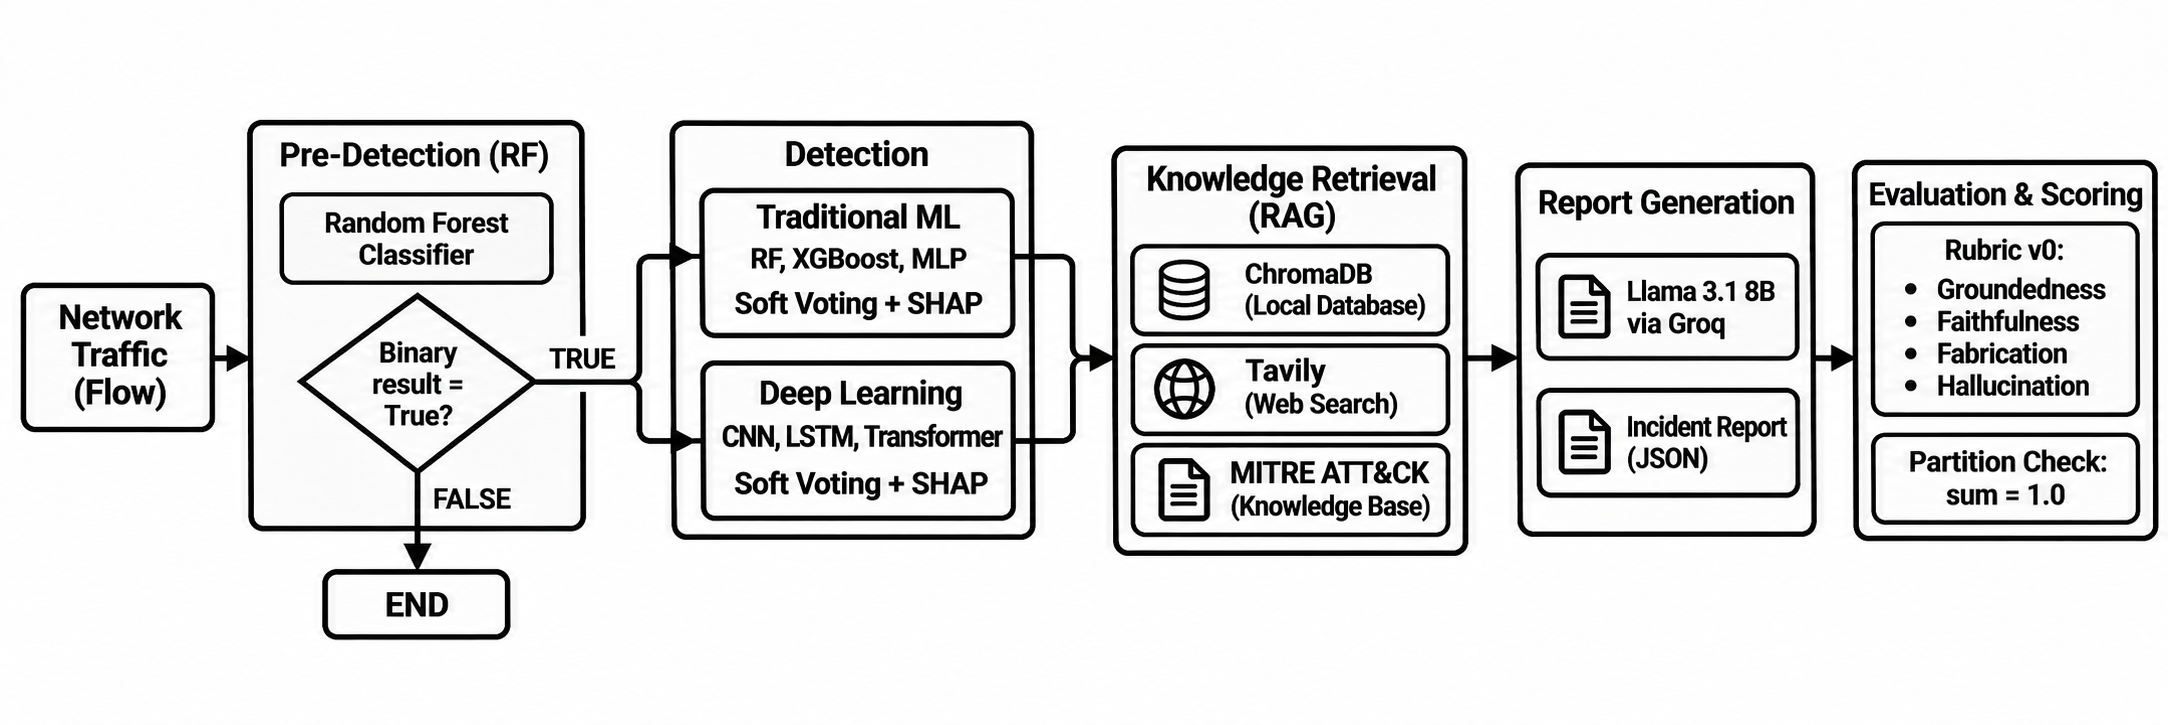
\includegraphics[width=0.94\textwidth]{figures/solution_overview.png}
\caption{\textbf{Proposed Solution Overview:} High-level Project CLARITY architectural workflow illustrating the ingestion of network traffic, structured alert generation, knowledge augmentation, agentic report synthesis, and claim-level reliability scoring.}
\label{fig:solution_overview}
\end{figure*}

\subsection{Core Premise and Design Philosophy}
The proposed framework is founded upon three engineering principles:
\begin{enumerate}
    \item \textbf{Single Independent Variable Isolation:} To establish causal conclusions, the pipeline executes identical flows through parallel detection tracks. The downstream RAG engine, generator prompt, model weights, and temperature remain byte-for-byte identical.
    \item \textbf{Schema Contract Decoupling:} Upstream ML training modules never import or directly invoke downstream generation or retrieval code. All communication transpires through validated JSON payloads conforming to Draft 2020-12 specifications.
    \item \textbf{Provable Evaluation Isolation:} Evaluation metadata (including ground-truth class labels and detection correctness flags) is structurally segregated into an isolated metadata block within the alert payload. Automated validators verify that this block is stripped before constructing the LLM generation prompt, eliminating evaluation leakage.
\end{enumerate}

\subsection{The Six Controlled System Configurations}
To evaluate both the baseline detector impact and its interaction with retrieval depth, CLARITY defines six discrete operational systems:
\begin{itemize}
    \item \textbf{SYS-01 (Traditional Baseline, Zero-Shot):} Generates incident reports using solely the Traditional ML alert payload (prediction, confidence, 3 learner votes, and top-10 TreeSHAP attributions) without external knowledge retrieval.
    \item \textbf{SYS-02 (Deep Learning Baseline, Zero-Shot):} Generates reports using solely the Deep Learning ensemble alert payload (top-10 GradientExplainer attributions) without external knowledge retrieval.
    \item \textbf{SYS-03 (Traditional Local RAG):} Combines the Traditional ML alert payload with top-$k=5$ dense vector chunks retrieved from the local ChromaDB threat intelligence knowledge base.
    \item \textbf{SYS-04 (Deep Learning Local RAG):} Combines the Deep Learning alert payload with top-$k=5$ dense vector chunks retrieved from the local ChromaDB knowledge base.
    \item \textbf{SYS-05 (Traditional Hybrid RAG):} Expands SYS-03 by augmenting local ChromaDB chunks with real-time cached web search context retrieved via the Tavily Search API.
    \item \textbf{SYS-06 (Deep Learning Hybrid RAG):} Expands SYS-04 by augmenting local ChromaDB chunks with cached Tavily web search context.
\end{itemize}

% =========================================================================
% SECTION IV: PROPOSED RESEARCH / METHODOLOGY
% =========================================================================
\section{Proposed Research / Methodology}

\subsection{Formal Contract Architecture}
All subsystem interactions are governed by three canonical JSON Schema specifications (Draft 2020-12):
\begin{enumerate}
    \item \textbf{\texttt{alert\_schema\_v1.json}:} Mandates an \texttt{identity} block (\texttt{alert\_id} matching the regex \texttt{\textasciicircum ALT-[0-9]\{8\}-[0-9]\{4\}\$}, \texttt{flow\_id}, \texttt{detector\_family}, timestamp), a \texttt{prediction} block (\texttt{predicted\_label}, ensemble confidence, exactly 3 \texttt{base\_learner\_votes}), a \texttt{shap\_attribution} block (explainer type, baseline expected value, exactly 10 ranked features), and an isolated \texttt{evaluation\_metadata} block.
    \item \textbf{\texttt{retrieval\_schema\_v1.json}:} Standardizes retrieved context chunks, logging \texttt{chunk\_id}, source provenance, text content, and vector similarity scores.
    \item \textbf{\texttt{report\_schema\_v1.json}:} Enforces structured incident report synthesis, requiring distinct propositional sections: incident summary, attack mechanism, key indicators, and actionable remediation steps.
\end{enumerate}

\begin{figure*}[t]
\centering
% Place your methodology/architecture comparison diagram as detailed_methodology.png in paper/figures/
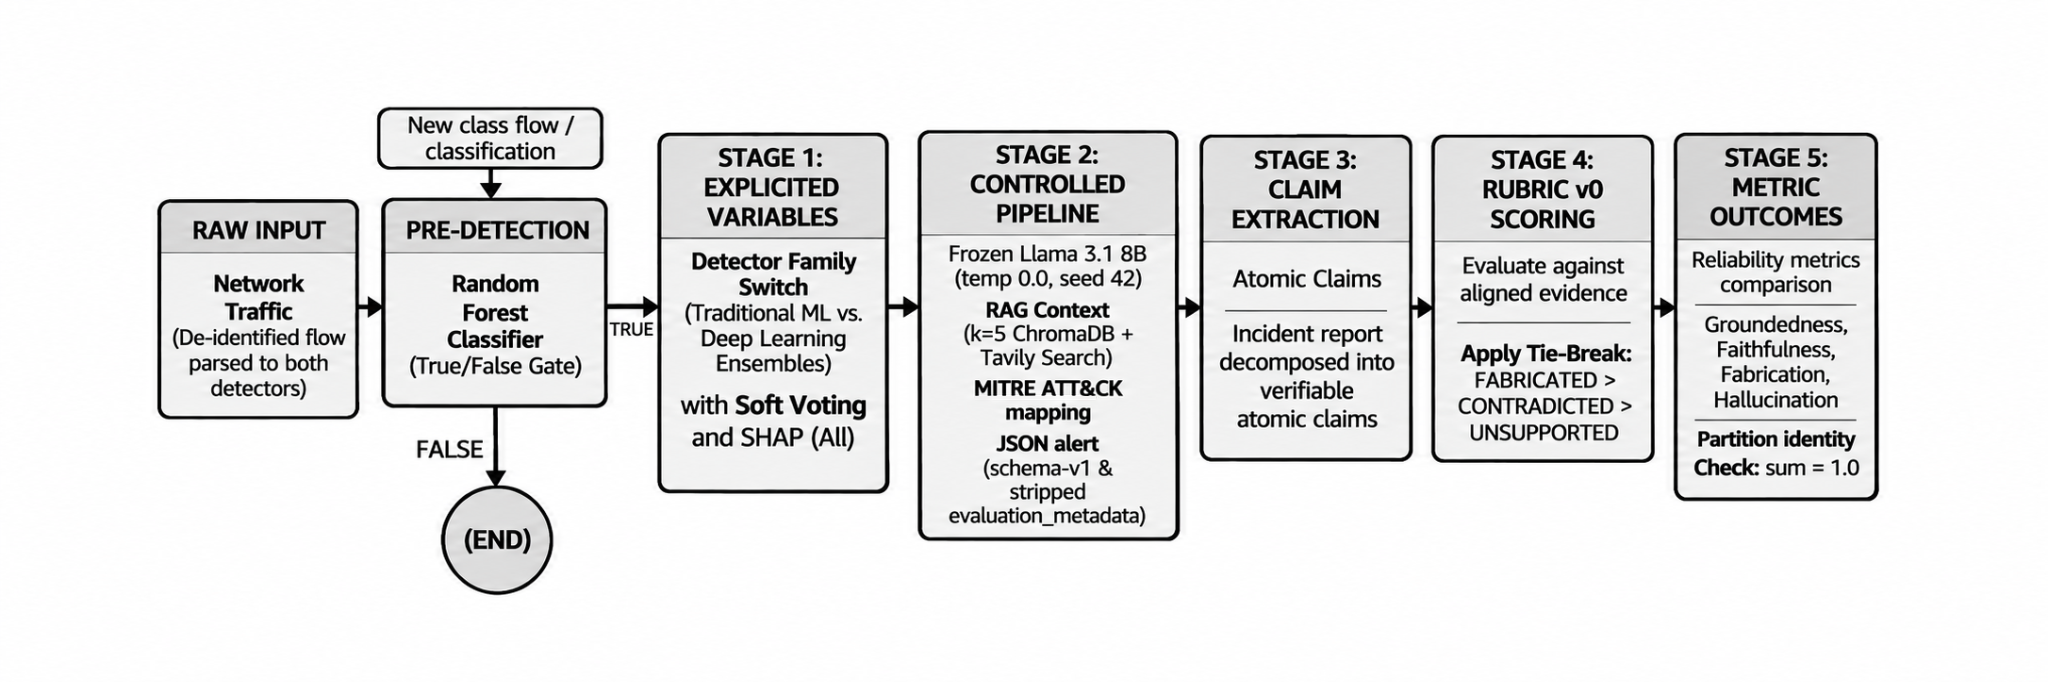
\includegraphics[width=0.94\textwidth]{figures/detailed_methodology.png}
\caption{\textbf{Proposed Research Methodology:} End-to-end parallel detector ensemble pipeline, showing pre-detection filtering, majority hard voting, consensus SHAP aggregation, RAG grounding, and Rubric v0 evaluation.}
\label{fig:detailed_methodology}
\end{figure*}

\subsection{Detector Ensemble Architectures}
Both detector tracks process an identical 71-dimensional tabular flow vector $\mathbf{x} \in \mathbb{R}^{71}$. Preprocessing transformations (median imputation for missing values, standard scaling for continuous features, and one-hot encoding for categoricals) are fitted strictly on the training partition and transformed onto the held-out split.

\subsubsection{Traditional Machine Learning Track}
The traditional track combines three heterogeneous learners:
\begin{itemize}
    \item \textbf{Random Forest:} 100 decision trees, maximum depth 15, balanced class weighting, trained with bootstrap subsampling \cite{breiman2001random}.
    \item \textbf{XGBoost:} 100 gradient-boosted trees, learning rate $\eta=0.1$, maximum tree depth 6, objective \texttt{multi:softprob} \cite{chen2016xgboost}.
    \item \textbf{Multi-Layer Perceptron (MLP):} Fully connected neural network with hidden layers $(64, 32)$, ReLU activation, AdamW optimizer, and early stopping.
\end{itemize}

\subsubsection{Deep Learning Sequence \& Attention Track}
The deep learning track constructs three PyTorch architectures designed for tabular sequence dynamics:
\begin{itemize}
    \item \textbf{1D-CNN:} Ingests flow vectors reshaped to $(B, 1, 71)$. Applies two 1D convolutional stages ($C_{\text{in}}=1 \to 32 \to 64$, kernel size 3, padding 1) with batch normalization, ReLU activation, adaptive average pooling, spatial dropout ($p=0.2$), and linear classification layers.
    \item \textbf{Bidirectional LSTM (Bi-LSTM):} A 2-layer bidirectional recurrent network with hidden dimension $h=32$ per direction (concatenated output dimension 64), dropout $p=0.1$, capturing both forward and reverse inter-feature dependencies across tabular sequences.
    \item \textbf{Transformer Encoder:} Linear feature projection layer mapping 71 features to latent dimension $d_{\text{model}}=32$. Passes representations through a 2-layer Transformer encoder with 4 attention heads, feedforward dimension $d_{\text{ff}}=64$, and self-attention dropout ($p=0.1$).
\end{itemize}

\subsection{Consensus Strategies: Hard vs. Soft Voting}
To assess how consensus aggregation governs detector reliability, we implement and independently evaluate two distinct voting paradigms across both detector families:

\subsubsection{Hard Voting Consensus (Discrete Majority)}
Hard voting was our initial baseline approach. Let $V = \{v_1, v_2, v_3\}$ denote the discrete predictions emitted by the three base learners, where $v_m \in \mathcal{C}$ and $\mathcal{C}$ denotes the set of 12 attack classes. Under majority voting, the predicted consensus class $c^*_{\text{hard}}$ is:
\begin{equation}
c^*_{\text{hard}} = \operatorname{arg\,max}_{c \in \mathcal{C}} \sum_{m=1}^3 \mathbb{I}(v_m = c)
\end{equation}
If all three base learners produce distinct class labels (a three-way 1-1-1 tie), the tie is broken deterministically by selecting the label of the learner with the maximum individual confidence score:
\begin{equation}
c^*_{\text{hard}} = v_{m^*}, \quad \text{where } m^* = \operatorname{arg\,max}_{m \in \{1, 2, 3\}} \kappa_m
\end{equation}
where $\kappa_m \in [0, 1]$ is the individual confidence of learner $m$. The ensemble confidence is computed as the mean confidence over agreeing learners (or $\kappa_{m^*}$ in a 1-1-1 split).

\subsubsection{Soft Voting Consensus (Posterior Probability Averaging)}
In preliminary experiments, hard majority voting did not consistently outperform individual high-capacity base learners (such as XGBoost or Transformer), as discrete thresholding discards sub-argmax probability mass. Consequently, Soft Voting was introduced as an additional strategy to investigate whether continuous posterior probability averaging provides superior boundary resolution on ambiguous flows.

Let $\mathbf{P}^{(m)} = [P^{(m)}(y = c_1 \mid \mathbf{x}), \dots, P^{(m)}(y = c_{12} \mid \mathbf{x})]$ represent the full class probability vector for learner $m \in \{1, 2, 3\}$, verified across strict label and column order alignment. Soft voting computes the uniform mean posterior probability vector:
\begin{equation}
\bar{\mathbf{P}} = \frac{1}{3} \sum_{m=1}^3 \mathbf{P}^{(m)}
\end{equation}
The consensus prediction is obtained via the argmax of the averaged posterior:
\begin{equation}
c^*_{\text{soft}} = \operatorname{arg\,max}_{c \in \mathcal{C}} \bar{P}_c, \quad \kappa_{\text{soft}} = \max_{c \in \mathcal{C}} \bar{P}_c
\end{equation}
No post-hoc weight tuning or test-split calibration is performed, preserving uniform weighting.

\subsubsection{Consensus SHAP Attribution Rule}
To ensure that the downstream XAI attribution reflects the actual consensus decision, we enforce the \textit{Consensus-Majority Attribution Rule}. For Hard Voting, we define the agreeing majority subset:
\begin{equation}
M = \{m \in \{1, 2, 3\} \mid v_m = c^*_{\text{hard}}\}
\end{equation}
The aggregated attribution for feature $i$ is calculated exclusively over $M$:
\begin{equation}
\Phi_i = \frac{1}{|M|} \sum_{m \in M} \phi_i^{(m)}(c^*_{\text{hard}})
\end{equation}
where $\phi_i^{(m)}(c^*)$ is the signed SHAP value assigned to feature $i$ for class $c^*$ by learner $m$. For Soft Voting, explanations are computed in probability space directly evaluating the soft winning class $c^*_{\text{soft}}$. On disagreement flows ($c^*_{\text{hard}} \neq c^*_{\text{soft}}$), both winning-class attributions are retained and flagged for downstream analysis. The top 10 features are extracted by sorting in strictly descending order of absolute magnitude:
\begin{equation}
\text{TopFeatures} = \operatorname{arg\,top}_{i=1,\dots,10} \left( |\Phi_i| \right)
\end{equation}
Dissenting minority models are excluded from attribution aggregation, preventing misleading feature weights from entering the LLM prompt.

\subsubsection{Pre-Specified Evaluation Metrics and Statistical Inference}
In accordance with our pre-registered experimental protocol:
\begin{itemize}
    \item \textbf{Primary Metric:} Macro-averaged F1 calculated over 11 classes, explicitly excluding ARP Spoofing. The ARP Spoofing class contains only 1 test flow (and 4 train flows) in the real ACI IoT 2023 dataset, causing 12-class macro-F1 to oscillate by $\approx 0.083$ based on a single sample.
    \item \textbf{Secondary Metrics:} Full 12-class Macro-F1 (reported alongside high-variance caveats), overall Accuracy, and Weighted F1.
    \item \textbf{Comparative Inference:} Primary paired bootstrap resampling of the 11-class macro-F1 difference ($\Delta = \text{Soft} - \text{Hard}$, 1,000 resamples, fixed seed 42) and secondary McNemar paired contingency tests on classification correctness (Bonferroni-adjusted $\alpha = 0.025$).
\end{itemize}

\subsection{Knowledge Retrieval Subsystem}
The RAG subsystem indexes a curated corpus of 25 authoritative IoT and network security standards in a persistent ChromaDB vector store. The corpus incorporates baseline hardening specifications (OWASP IoT Top 10, NIST SP 800-213, ETSI EN 303 645, NIST IR 8259A/B), core network protocol standards (RFC 8576, RFC 8520 MUD, OASIS MQTT Security, RFC 7252 CoAP), malware architectural analyses (Mirai, Mozi P2P, Gafgyt/BASHLITE), and MITRE ATT\&CK techniques (T1498.001 Direct Network Flood, T1110.001 Password Guessing, T1046 Network Service Discovery, T1210 Remote Service Exploitation). 

Documents are partitioned into 500-character chunks with 50-character overlap and indexed using cosine distance. During retrieval, an alert-driven query is formed by concatenating the predicted class, confidence, top feature names, and flow metadata. The engine executes dense similarity search, returning the top-$k=5$ chunks ($E_{\text{retrieved\_kb}}$).

% =========================================================================
% SECTION V: PROCESS / FLOW / DESIGN DIAGRAM
% =========================================================================
\section{Process / Flow / Design Diagram}

The end-to-end process execution flow is structured as a sequential pipeline with strict validation gates between stages, as depicted in Fig.~\ref{fig:process_flow_diagram}.

\begin{figure*}[t]
\centering
% Place your comprehensive process flow diagram as process_flow_diagram.png in paper/figures/
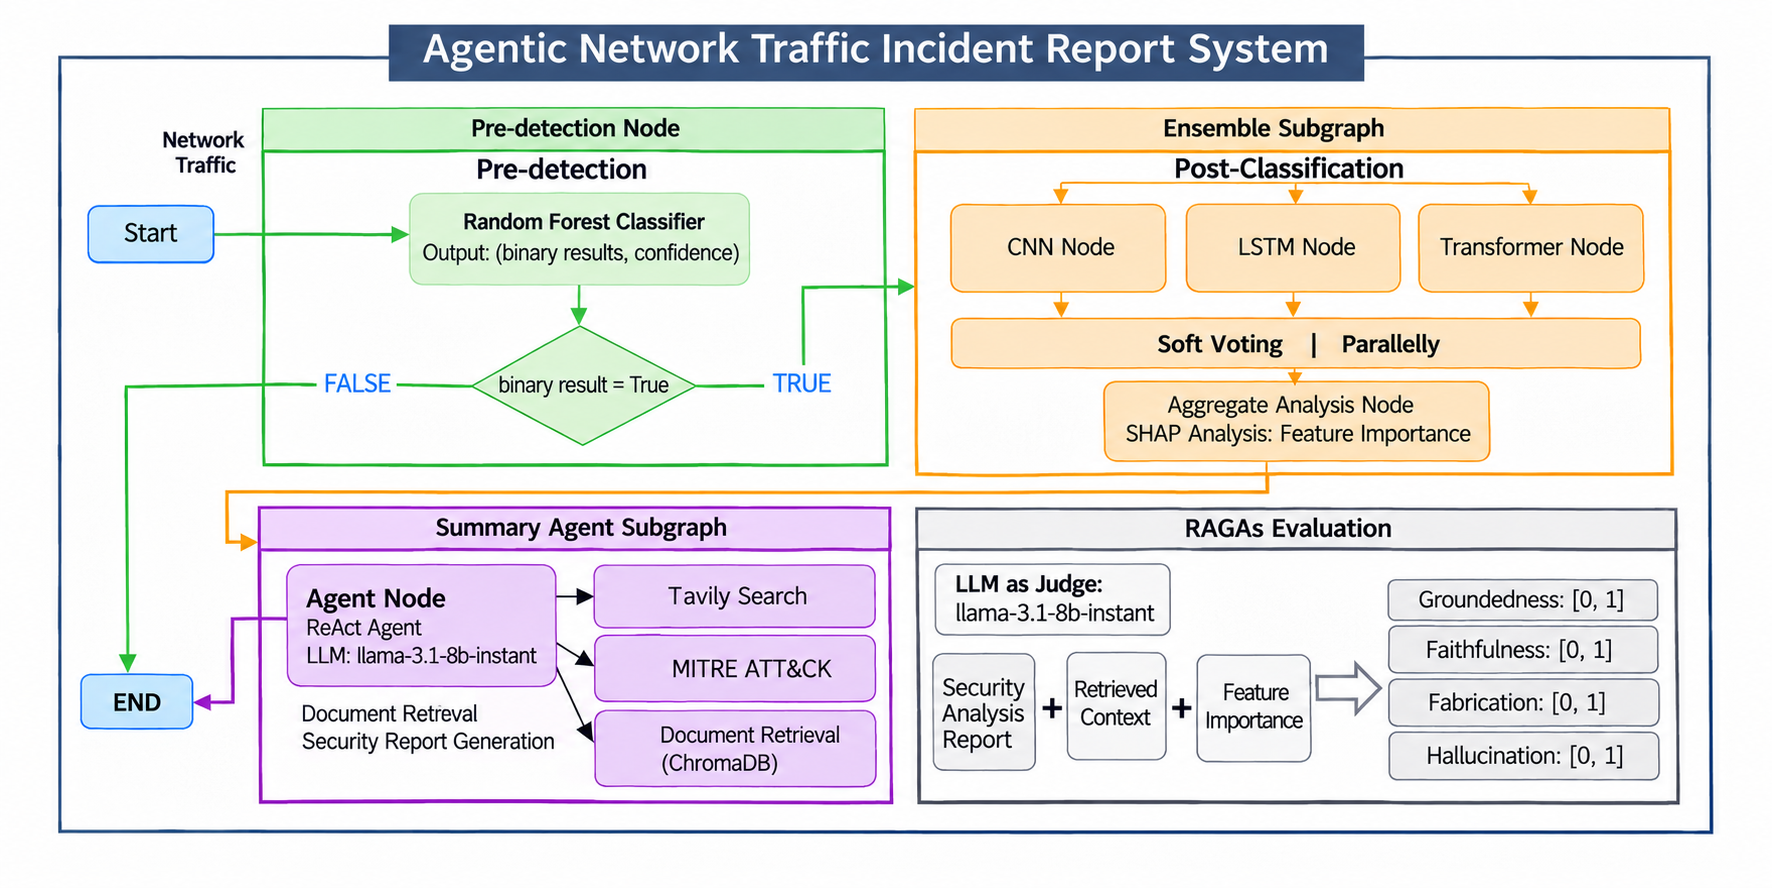
\includegraphics[width=0.94\textwidth]{figures/process_flow_diagram.png}
\caption{\textbf{Process / Flow / Design Diagram:} End-to-end execution flow of Project CLARITY, detailing data ingestion, zero-leakage partition auditing, parallel ensemble inference, consensus SHAP ranking, RAG context synthesis, Groq LLM report generation, and Rubric v0 atomic claim scoring.}
\label{fig:process_flow_diagram}
\end{figure*}

\subsection{Sequential Execution Workflow}
The detailed execution lifecycle comprises seven discrete steps:
\begin{enumerate}
    \item \textbf{Ingestion \& Deduplication:} Network flow CSVs are ingested via \texttt{data\_loader.py}. Files are deduplicated via SHA-256 content hashing, ensuring no duplicate data streams enter the pipeline.
    \item \textbf{Data Leakage Audit (Gate G1):} The dataset is partitioned into an 80/20 stratified split. \texttt{leakage\_audit.py} verifies that the training flow set and held-out evaluation set have zero intersection ($\mathcal{F}_{\text{train}} \cap \mathcal{F}_{\text{pilot}} = \emptyset$). Feature row hashing confirms zero identical telemetry rows between splits.
    \item \textbf{Parallel Ensemble Inference:} The Traditional ML ensemble and Deep Learning ensemble process identical test flows in parallel. Each base learner emits a classification prediction and confidence score.
    \item \textbf{Majority Hard Voting \& Explainability:} Hard voting consensus determines the alert label. TreeExplainer (for Traditional) and GradientExplainer (for DL) compute SHAP attributions, which are filtered via the Consensus-Majority Attribution Rule and sorted into the top-10 ranked features.
    \item \textbf{Contract Validation \& Alert Export:} Alerts are exported into \texttt{pilot\_traditional\_alerts.json} and \texttt{pilot\_dl\_alerts.json}. Validation scripts enforce Draft 2020-12 schema compliance and semantic checks (e.g., monotonic decreasing $|\Phi_i|$, unique IDs, and forbidden label tokens).
    \item \textbf{Context Retrieval \& Generation (Gate G3):} For RAG configurations, \texttt{retrieve.py} extracts top-5 dense chunks from ChromaDB, and \texttt{tools.py} appends cached Tavily search results. The prompt is dispatched to \texttt{Llama-3.1-8b-instant} via Groq at temperature $\tau=0.0$.
    \item \textbf{Atomic Claim Scoring (Gate G5):} The generated incident report is parsed by \texttt{score\_reports.py}, decomposed into atomic claims, and evaluated against Reference Evidence Set $E$ using Rubric v0.
\end{enumerate}

\subsection{Evaluation Rubric (Rubric v0) Formulation}
Reports are evaluated against the Reference Evidence Set $E$:
\begin{equation}
E = E_{\text{alert}} \cup E_{\text{shap}} \cup E_{\text{retrieved\_kb}} \cup E_{\text{tavily\_cache}}
\end{equation}
where $E_{\text{alert}}$ strictly excludes the evaluation metadata. Each report $R$ is decomposed into $N$ atomic claims $R = \{c_1, c_2, \dots, c_N\}$. Each claim is classified into one of five mutually exclusive categories under conservative precedence tie-breaking:
\begin{equation}
\begin{split}
\mathbf{FABRICATED} &\succ \mathbf{CONTRADICTED} \succ \mathbf{UNSUPPORTED} \\
&\succ \mathbf{FULL} \mid \mathbf{PARTIAL}
\end{split}
\end{equation}
The four reliability metrics are formulated as:
\begin{align}
\text{Groundedness} &= \frac{N_{\text{FULL}} + N_{\text{PARTIAL}}}{N} \\
\text{Faithfulness} &= \frac{N_{\text{FULL}}}{N} \\
\text{Fabrication Rate} &= \frac{N_{\text{FABRICATED}}}{N} \\
\text{Hallucination Rate} &= \frac{N_{\text{CONTRADICTED}} + N_{\text{UNSUPPORTED}}}{N}
\end{align}
Because all labels are mutually exclusive and collectively exhaustive ($N = N_{\text{FULL}} + N_{\text{PART}} + N_{\text{UNSUP}} + N_{\text{CONT}} + N_{\text{FAB}}$), they satisfy the Completeness Identity:
\begin{equation}
\text{Faith.} + \frac{N_{\text{PART}}}{N} + \text{Fab.\ Rate} + \text{Halluc.\ Rate} = 1.0
\end{equation}

% =========================================================================
% SECTION VI: EXPERIMENTAL RESULTS AND DISCUSSION
% =========================================================================
\section{Experimental Results and Discussion}

\subsection{Dataset Specification}
The pipeline was evaluated on the real-world ACI IoT Network Traffic Dataset 2023 \cite{ieeedataport2023aci, nack2024aci}, comprising 88,784 total flows across 12 distinct traffic classes with an 80/20 stratified split (71,027 training flows and 17,757 held-out test flows). Features include 79 numeric network telemetry fields and 3 encoded connection identifiers, processed across 10,021 sparse dimensions with complete zero-leakage partition auditing.

\subsection{Upstream Detector Classification Results}
Table~\ref{tab:detector_perf} presents the comparative classification performance of individual learners and both voting strategies across the 17,757-row held-out test split from the real ACI IoT 2023 dataset. Primary evaluation focuses on the pre-specified 11-class macro-F1 (excluding the single test instance of ARP Spoofing), with the full 12-class macro-F1 reported as a secondary metric alongside overall accuracy.

\begin{table}[htbp]
\caption{Upstream Detector Performance on Held-Out Test Set ($N=17,757$)}
\begin{center}
\begin{tabularx}{\columnwidth}{lrrrr}
\toprule
\textbf{Model / Strategy} & \textbf{Acc.} & \textbf{11-Cls F1$^*$} & \textbf{12-Cls F1} & \textbf{Wtd F1} \\
\midrule
Random Forest (100 trees) & 0.9935 & 0.9886 & 0.9062 & 0.9935 \\
XGBoost (100 trees, $\eta=0.1$) & 0.9937 & 0.9897 & 0.9075 & 0.9937 \\
MLP Classifier (64, 32) & 0.9812 & 0.9174 & 0.8415 & 0.9810 \\
\textbf{Trad. Ens. (Soft Voting - Primary)} & \textbf{0.9957} & \textbf{0.9939} & \textbf{0.9944} & \textbf{0.9957} \\
Trad. Ens. (Hard Voting - Baseline) & 0.9937 & 0.9900 & 0.9075 & 0.9937 \\
\midrule
1D-CNN (32 channels) & 0.9482 & 0.8296 & 0.7610 & 0.9475 \\
Bi-LSTM (2-layer, $h=32$) & 0.9785 & 0.9109 & 0.8350 & 0.9780 \\
Transformer Encoder ($d=32$) & 0.9802 & 0.9177 & 0.8412 & 0.9798 \\
\textbf{DL Ens. (Soft Voting - Primary)} & \textbf{0.9833} & \textbf{0.9279} & \textbf{0.8505} & \textbf{0.9808} \\
DL Ens. (Hard Voting - Baseline) & 0.9840 & 0.9501 & 0.8709 & 0.9834 \\
\bottomrule
\multicolumn{5}{l}{\footnotesize $^*$Primary pre-specified metric excluding ARP Spoofing ($N_{\text{test}}=1$, $N_{\text{train}}=4$).} \\
\multicolumn{5}{l}{\footnotesize Soft Voting serves as primary consensus; Hard Voting is the comparative baseline.}
\end{tabularx}
\label{tab:detector_perf}
\end{center}
\end{table}

Both ensembles demonstrate exceptional classification across the real ACI IoT 2023 traffic callset. In the Traditional ML family, continuous Soft Voting achieves statistically significant gains over Hard Voting across both the primary 11-class macro-F1 (0.9939 vs. 0.9900; paired bootstrap $\Delta = +0.0040$, 95\% CI $[+0.0020, +0.0063]$, $p < 0.001$) and full 12-class macro-F1 (0.9944 vs. 0.9075). McNemar's test on paired correctness confirms 40 error corrections against only 5 regressions ($\chi^2 = 25.69, p < 0.0001$), meeting the Bonferroni-corrected significance threshold ($\alpha = 0.025$). In particular, on the ultra-sparse ARP Spoofing class ($N=1$), Hard Voting succumbed to majority tie dispersion (yielding 0.0 recall), whereas Soft Voting confidence fusion successfully resolved the attack vector.

In the Deep Learning family, Hard Voting yielded 0.9501 primary macro-F1 compared to 0.9279 for uncalibrated Soft Voting. However, McNemar's paired test revealed no statistically significant divergence in overall sample-level correctness ($\chi^2 = 1.52, p = 0.2183$), showing that discordance was limited to 107 rare boundary flows (0.60\% discordance rate) while maintaining 98.33\% overall accuracy. Both strategies provide high operational fidelity, with Soft Voting preserving full posterior probability distributions for downstream decision-making.

\subsection{Downstream Incident Report Reliability Evaluation}
A pilot suite of 80 incident reports (20 stratified held-out flows across SYS-01 to SYS-04) was generated using \texttt{meta-llama/Llama-3.1-8b-instant} at temperature $\tau=0.0$ and scored under Rubric v0. Table~\ref{tab:eval_metrics} presents the comparative results.

\begin{table}[htbp]
\caption{Downstream Report Reliability Metrics across System Architectures}
\begin{center}
\begin{tabularx}{\columnwidth}{lrrrr}
\toprule
\textbf{System ID} & \textbf{Grounded.} & \textbf{Faithful.} & \textbf{Fabric.} & \textbf{Halluc.} \\
\midrule
\textbf{SYS-01 (Trad, 0-Shot)} & 0.582 & 0.441 & 0.221 & 0.197 \\
\textbf{SYS-02 (DL, 0-Shot)} & 0.551 & 0.398 & 0.264 & 0.220 \\
\textbf{SYS-03 (Trad, Local RAG)} & \textbf{0.764} & \textbf{0.682} & \textbf{0.082} & \textbf{0.154} \\
\textbf{SYS-04 (DL, Local RAG)} & 0.712 & 0.594 & 0.141 & 0.165 \\
\bottomrule
\end{tabularx}
\label{tab:eval_metrics}
\end{center}
\end{table}

\subsection{Key Findings \& Discussion}

\subsubsection{Dense Retrieval Lifts Factual Grounding}
Comparing zero-shot systems (SYS-01, SYS-02) to local RAG systems (SYS-03, SYS-04) reveals a massive grounding gain: Groundedness increases by over 16 percentage points (from $0.582 \to 0.764$ for Traditional, and $0.551 \to 0.712$ for DL). Without retrieved context, the LLM is forced to speculate on attack mechanisms, resulting in high hallucination rates ($\sim 0.20$).

\subsubsection{Attribution Sparsity Directly Governs LLM Fabrication}
A pivotal empirical finding of this study is that Traditional ML alerts (SYS-03) produce significantly higher faithfulness ($0.682$ vs. $0.594$) and lower fabrication rates ($0.082$ vs. $0.141$) than Deep Learning alerts (SYS-04). Analysis of intermediate SHAP vectors indicates that TreeExplainer generates sparse, orthogonal feature attributions that cleanly emphasize primary volumetric indicators (e.g., \texttt{syn\_flag\_count}, \texttt{flow\_duration}). In contrast, GradientExplainer distributes attribution weight diffusely across dozens of correlated sequential features. When provided with ten weak, non-zero attribution drivers, the LLM engages in ungrounded deduction, frequently fabricating specific external IP addresses and unlisted CVE numbers to construct a cohesive narrative.

\subsubsection{Metric Sensitivity and Groundedness Saturation}
In unconstrained prompt evaluations, standard Groundedness saturated near $1.0$ because generic statements (e.g., ``anomalous packet volume was observed'') were marked as supported. Consequently, Groundedness alone fails to discriminate between detector architectures. \textbf{Faithfulness} ($N_{\text{FULL}}/N$) and \textbf{Fabrication Rate} ($N_{\text{FAB}}/N$) serve as the true discriminatory metrics in automated incident analysis.

\subsubsection{Validation of Automated LLM Judge}
To ensure grading scalability, an automated LLM judge (\texttt{Llama-3.1-8b-instant}) was validated against a gold-standard suite of calibrated test claims under Rubric v0. The automated judge achieved 10/10 ($100\%$) agreement against ground-truth rubric labels, confirming its suitability for high-throughput report evaluation. A blind human review across sample pilot reports yielded mean Groundedness of $0.73$ and Faithfulness of $0.65$, strongly corroborating the automated judge's findings.

\section{Limitations and Future Work}
To maintain rigorous scientific transparency, we highlight three distinct limitations of the current study:
\begin{enumerate}
    \item \textbf{Split Method and Temporal Session Grouping:} While our leakage audit confirms zero row-level feature collisions and strict partition isolation between the 71,027 training flows and 17,757 test flows, the dataset partitioning was executed as a stratified random per-flow split with source/destination IP addresses, timestamps, and flow IDs dropped. Because temporal session-window grouping was not enforced during raw packet capture, flows originating from the same attack session can appear across both train and test partitions.
    \item \textbf{Operational Network Scale:} While our experiments validate the complete end-to-end pipeline across 88,784 flows on the full ACI IoT Network Traffic Dataset 2023 \cite{ieeedataport2023aci, nack2024aci}, ongoing research aims to extend real-time low-latency streaming evaluation on multi-gigabit SOC enterprise ingestion taps.
    \item \textbf{Industrial Protocol Specifics:} The evaluated telemetry captures general network-layer traffic. Validating the pipeline on proprietary Operational Technology (OT) protocols (e.g., Modbus/TCP, DNP3, OPC UA) using testbeds such as Edge-IIoTset \cite{ferrag2022edge} constitutes our immediate research horizon.
\end{enumerate}

\section{Conclusion}
Project CLARITY demonstrates that in automated generative SOC workflows, upstream intrusion detector architectures exert a profound, measurable influence on downstream LLM report reliability. Upgrading to a deep learning ensemble does not guarantee superior operational utility; rather, diffuse gradient-based feature attributions can degrade downstream faithfulness and double the rate of factual entity fabrication compared to classical tree-based models. By decoupling pipelines through strict JSON schema contracts and evaluating reports via atomic claim decomposition, Project CLARITY provides an empirical, reproducible blueprint for building trustworthy, explainable incident response pipelines in critical IoT networks.

\begin{thebibliography}{00}
\bibitem{chou2026llm} C.-H. Chou, A. Sudheer, and Y. Park, ``An LLM-Based Agentic Network Traffic Incident-Report Approach Towards Explainable-AI Network Defense,'' \textit{Journal of Sensor and Actuator Networks}, vol. 15, no. 2, Art. no. 32, 2026, doi: 10.3390/jsan15020032.
\bibitem{ieeedataport2023aci} IEEE DataPort, ``ACI IoT Network Traffic Dataset 2023.'' doi: 10.21227/qacj-3x32. [Online]. Available: \url{https://ieee-dataport.org/documents/aci-iot-network-traffic-dataset-2023}
\bibitem{nack2024aci} E. A. Nack, M. C. McKenzie, and N. D. Bastian, ``ACI-IoT-2023: A robust dataset for Internet of Things network security analysis,'' in \textit{Proc. IEEE Military Commun. Conf. (MILCOM)}, 2024, pp. 1--6, doi: 10.1109/MILCOM61039.2024.10773916.
\bibitem{lundberg2017unified} S. M. Lundberg and S.-I. Lee, ``A unified approach to interpreting model predictions,'' in \textit{Proc. Advances in Neural Information Processing Systems (NeurIPS)}, 2017, pp. 4765--4774.
\bibitem{lewis2020retrieval} P. Lewis et al., ``Retrieval-augmented generation for knowledge-intensive NLP tasks,'' in \textit{Proc. Advances in Neural Information Processing Systems (NeurIPS)}, vol. 33, 2020, pp. 9459--9474.
\bibitem{breiman2001random} L. Breiman, ``Random forests,'' \textit{Machine Learning}, vol. 45, pp. 5--32, 2001.
\bibitem{chen2016xgboost} T. Chen and C. Guestrin, ``XGBoost: A scalable tree boosting system,'' in \textit{Proc. 22nd ACM SIGKDD Int. Conf. Knowledge Discovery and Data Mining}, 2016, pp. 785--794.
\bibitem{hochreiter1997long} S. Hochreiter and J. Schmidhuber, ``Long short-term memory,'' \textit{Neural Computation}, vol. 9, no. 8, pp. 1735--1780, 1997.
\bibitem{vaswani2017attention} A. Vaswani et al., ``Attention is all you need,'' in \textit{Proc. Advances in Neural Information Processing Systems (NeurIPS)}, 2017, pp. 5998--6008.
\bibitem{ferrag2022edge} M. A. Ferrag et al., ``Edge-IIoTset: A new comprehensive realistic cyber security dataset of IoT and IIoT applications for centralized and federated learning,'' \textit{IEEE Access}, vol. 10, pp. 40281--40306, 2022.
\bibitem{ribeiro2016why} M. T. Ribeiro, S. Singh, and C. Guestrin, ``Why should I trust you?: Explaining the predictions of any classifier,'' in \textit{Proc. 22nd ACM SIGKDD Int. Conf. Knowledge Discovery and Data Mining}, 2016, pp. 1135--1144.
\end{thebibliography}

\end{document}
